\documentclass[11pt, oneside, titlepage]{article}
\usepackage[letterpaper, margin=2cm]{geometry}
\usepackage{MATH517}
\usepackage{Calculus}

\title{MATH 517 Finite Differences Homework 6}
\author{Caleb Logemann}

\begin{document}
\maketitle

%\lstinputlisting[language=Matlab]{H01_23.m}
\begin{enumerate}
    \item % #1
        Consider the following method for solving the heat equation $u_t = u_{xx}$:
        \[
            U^{n+2}_i = U^n_i + \frac{2k}{h^2}\p{U^{n+1}_{i-1} - 2U^{n+1}_i + U^{n+1}_{i+1}}
        \]
        \begin{enumerate}
            \item[(a)] % Done
                Determine the order of accuracy of this method (in both space
                and time).

                In order to find the order of accuracy of this method, the
                local truncation error for this method must be found.
                The local truncation error for this method is given as
                \begin{align*}
                    \tau &= \frac{1}{2k}\p{u(t + k, x) - u(t - k, x)} - \frac{1}{h^2}
                        \p{u(t, x-h) - 2u(t, x) + u(t, x+h)}
                \end{align*}
                I will consider the time and space terms seperately at first
                \begin{gather*}
                    u(t + k, x) = u(t, x) + k u_t(t, x) + \frac{1}{2} k^2 u_{tt}(t, x) + \frac{1}{6}k^3 u_{ttt}(t, x) + O(k^4) \\
                    u(t - k, x) = u(t, x) - k u_t(t, x) + \frac{1}{2} k^2 u_{tt}(t, x) - \frac{1}{6}k^3 u_{ttt}(t, x) + O(k^4) \\
                    \frac{1}{2k}\p{u(t + k, x) - u(t - k, x)} = \frac{1}{2k}\p{2k u_t(t, x) + \frac{1}{3}k^3 u_{ttt}(t, x) + O(k^4)} \\
                    \frac{1}{2k}\p{u(t + k, x) - u(t - k, x)} = u_t(t, x) + \frac{1}{6}k^2 u_{ttt}(t, x) + O(k^3) \\
                    u(t, x-h) = u(t, x) - h u_x(t, x) + \frac{1}{2} h^2 u_{xx}(t, x) - \frac{1}{6} h^3 u_{xxx}(t, x) + \frac{1}{24} h^4 u_{xxxx}(t, x) + O(h^5) \\
                    u(t, x+h) = u(t, x) + h u_x(t, x) + \frac{1}{2} h^2 u_{xx}(t, x) + \frac{1}{6} h^3 u_{xxx}(t, x) + \frac{1}{24} h^4 u_{xxxx}(t, x) + O(h^5) \\
                    \frac{1}{h^2}\p{u(t, x-h) - 2u(t, x) + u(t, x+h)} = \frac{1}{h^2} \p{h^2 u_{xx}(t, x) + \frac{1}{12} h^4 u_{xxxx} + O(h^6)} \\
                    \frac{1}{h^2}\p{u(t, x-h) - 2u(t, x) + u(t, x+h)} = u_{xx}(t, x) + \frac{1}{12} h^2 u_{xxxx} + O(h^4)
                \end{gather*}
                Note that in the spacial terms the 5th order error canceled out.

                Using these two expressions the full truncation error is
                \begin{align*}
                    \tau &= u_t(t, x) + \frac{1}{6}k^2 u_{ttt}(t, x) + O(k^3) - u_{xx}(t, x) - \frac{1}{12} h^2 u_{xxxx} + O(h^4) \\
                    \intertext{The heat equation states that $u_t(t, x) = u_{xx}(t, x)$}
                    \tau &= \frac{1}{6}k^2 u_{ttt}(t, x) + O(k^3) - u_{xx}(t, x) - \frac{1}{12} h^2 u_{xxxx} + O(h^4) \\
                    \tau &= O(k^2 + h^2)
                \end{align*}

            \item[(b)]
                Suppose we take $k = \alpha h^2$ for some fixed $\alpha > 0$
                and refine the grid.
                For what values of $\alpha$ will this method be Lax-Richtmyer
                stable and hence convergent?

            \item[(c)]
                Is this method useful?
        \end{enumerate}

    \item % #2 Done
        Consider the one-dimensional heat equation:
        \begin{align*}
            PDE &: u_t = \kappa u_{xx}\text{ for } (t, x) \in \br{0, T} \times \br{0, 1} \\
            BCs &: u(t, 0) = g_0, \; u(t, 1) = g_1 \\
            ICs &: u(0, x) = f(x)
        \end{align*}
        \begin{enumerate}
            \item[(a)] % Done
                The m-file heat\_CN.m solves the heat equation
                $u_t = \kappa u_{xx}$ using the Crank-Nicolson method.
                Run this code and by changing the number of grid points,
                confirm that it is second order accurate.
                Create a table of errors for varius h values, and $k = 4h$ at
                $T = 1$.

                The following script creates a table that verifies that the
                Crank-Nicolson is second order accurate.
                \lstinputlisting[language=Matlab, lastline=12]{H06.m}
                \begin{verbatim}
                    ans = 

                        hRatios    errorRatios    order 
                        _______    ___________    ______

                        2          8.1811         3.0323
                        2          4.4039         2.1388
                        2           3.999         1.9996
                        2          3.9953         1.9983
                        2               4              2
                        2               4              2
                        2               4              2
                \end{verbatim}

            \item[(b)] % Done
                The follwing method implements the TR-BDF2 method.
                \lstinputlisting[language=Matlab]{heat_trbdf2.m}
                The order of accuracy is checked with this script.
                \lstinputlisting[language=Matlab, firstline=14, lastline=25]{H06.m}

                The method is second order accurate as is shown below.
                \begin{verbatim}
                    ans = 

                        hRatios    errorRatios    order 
                        _______    ___________    ______

                        2          4.0302         2.0109
                        2          3.9812         1.9932
                        2          3.9898         1.9963
                        2           3.986         1.9949
                        2          3.9943         1.9979
                \end{verbatim}

                The boundary conditions were chosen based on the formulation
                of the TR-BDF2 method in section 8.5 of the book.
                For the first stage the boundaries of $U^n$ are given by
                $g(t = t^n, x = 0, 1)$.
                The boundaries of $U^*$ are given by $g(t = t^n + k/2, x = 0,1)$,
                because $U^*$ is an approximation of the solution at time $t = t^n + k/2$.
                Finally the boundaries of $U^{n+1}$ are given by
                $g(t = t^n + k = t^{n+1}, x = 0,1)$
        \end{enumerate}

    \item % #3 Done
        Again, consider the 1D heat equation.
        \begin{enumerate}
            \item[(a)] % Done
                \begin{enumerate}
                    \item[(i)]
                        The following function uses the new 
                        \lstinputlisting[language=Matlab]{heat_CN3.m}
                        This graph is after one time step, and shows that the
                        decay of the high wave numbers is not captured well.
                        \begin{center}
                            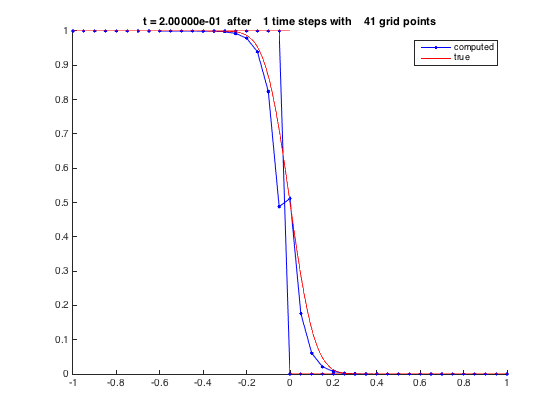
\includegraphics[scale=.7]{Figures/06_3_1.png}
                        \end{center}

                    \item[(ii)]
                        If $k = .1 h$ instead this high frequency is damped out
                        well, so that the high frequency modes present in part
                        (i) are no longer a problem.

                        However there is a problem with the accuracy when $m$ is odd.
                        When $m$ is odd the accuracy is severely limited because the
                        initial data is not symmetrical.
                        As is evident in the image below, the blue initial data
                        does not capture the discontinuity well.
                        At $x = 0$, the discretization is 0, however the point
                        directly to the left of $x = 0$ is skewing the initial data to
                        the left.
                        This causes the approximate solution to always be less than the
                        true solution.
                        \begin{center}
                            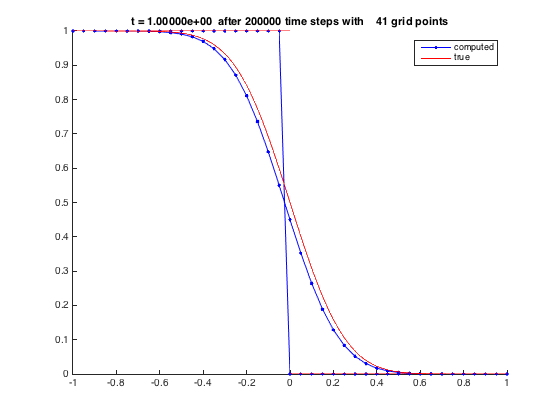
\includegraphics[scale=.7]{Figures/06_3_2.png}
                        \end{center}
                        If $m$ is even, then initial data become symmetrical around
                        $x = 0$, because there is no discritization point at $x = 0$.
                        This result in the following image.
                        \begin{center}
                            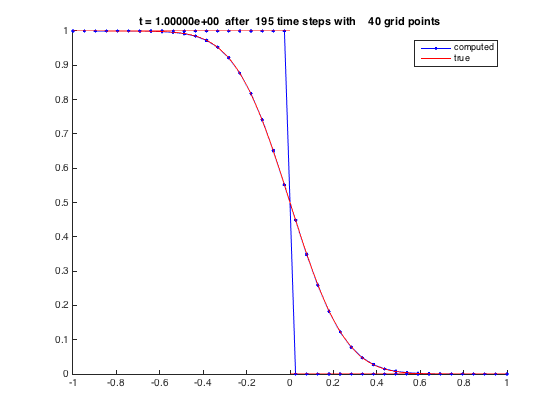
\includegraphics[scale=.7]{Figures/06_3_3.png}
                        \end{center}

                        The order of accuracy can be checked to be second order
                        as well with the following script.
                        \lstinputlisting[language=Matlab, firstline=27, lastline=39]{H06.m}
                        \begin{verbatim}
                            ans = 

                                hRatios    errorRatios    order 
                                _______    ___________    ______

                                1.9744     3.8904         1.9971
                                1.987      3.949         2.0003
                                1.9935     3.9746         2.0003
                                1.9967     3.9872         2.0001
                        \end{verbatim}
                \end{enumerate}

            \item[(b)] % Done
                The modified version of the trbdf2 method for solving this
                problem is shown below.
                \lstinputlisting[language=Matlab]{heat_trbdf23.m}
                With $k = 4h$ the order is shown below.
                \lstinputlisting[language=Matlab, firstline=40]{H06.m}
                \begin{verbatim}
                    ans = 

                        hRatios    errorRatios    order 
                        _______    ___________    ______

                        1.9744     3.9894          2.034
                        1.987     3.8007         1.9445
                        1.9935     3.9826         2.0032
                        1.9967     3.9902         2.0012
                \end{verbatim}

                This method is better than the Crank-Nicolson for this problem,
                because this method is L-stable.
                This method damps out high frequencies caused by the discontinuity
                much better than the CN method.
                This allows for the timestep to be much larger, while
                still maintaining the same accuracy.
                Since the timestep is larger, this method is much faster.
                The damping of high frequency modes can be seen by the
                following plot.
                \begin{center}
                    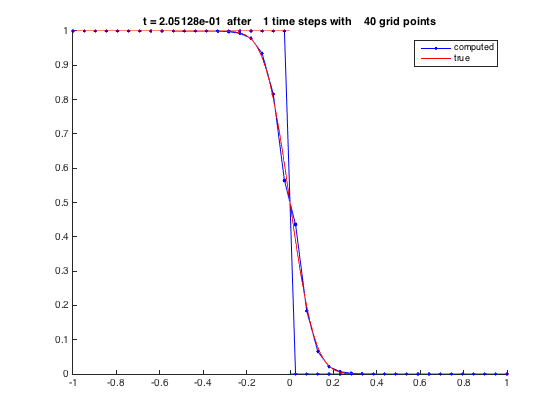
\includegraphics[scale=.7]{Figures/06_3_4.png}
                \end{center}
                The equivalent to this plot is shown in 3(a)(i).
                The high frequency is much less evident for this method, then the
                CN method.
        \end{enumerate}

    \item % #4
        Consider the following scheme for solving the 1D heat equation:
        \[
            U_j^{n+1} = U_j^{n-1} + \frac{2k}{h^2}
            \p{U^n_{j+1} - \p{U^{n+1}_j + U^{n-1}_j} + U^n_{j-1}}
        \]
        \begin{enumerate}
            \item[(a)]
                Determine the local truncation error of this scheme.

                The local truncation error for this scheme is given by
                \[
                    \tau = \frac{1}{2k}\p{u(t+k, x) - u(t-k, x)} - \frac{1}{h^2}\p{u(t, x+h) -
                        \p{u(t+k, x) + u(t-k, x)} + u(t, x-h)}
                \]
                We have shown previously in problem 1(a) that
                \[
                    \frac{1}{2k}\p{u(t+k, x) - u(t-k, x)} = u_t(t, x) + \frac{1}{6}k^2 u_{ttt}(t, x) + O(k^3). \\
                \]
                We can now consider the second term
                \begin{align*}
                    u(t, x-h) &= u(t, x) - h u_x(t, x) + \frac{1}{2} h^2 u_{xx}(t, x) - \frac{1}{6} h^3 u_{xxx}(t, x) + \frac{1}{24} h^4 u_{xxxx}(t, x) + O(h^5) \\
                    u(t, x+h) &= u(t, x) + h u_x(t, x) + \frac{1}{2} h^2 u_{xx}(t, x) + \frac{1}{6} h^3 u_{xxx}(t, x) + \frac{1}{24} h^4 u_{xxxx}(t, x) + O(h^5) \\
                    u(t+k, x) &= u(t, x) + k u_t(t, x) + \frac{1}{2} k^2 u_{tt}(t, x) + \frac{1}{6}k^3 u_{ttt}(t, x) + O(k^4) \\
                    u(t-k, x) &= u(t, x) - k u_t(t, x) + \frac{1}{2} k^2 u_{tt}(t, x) - \frac{1}{6}k^3 u_{ttt}(t, x) + O(k^4)
                \end{align*}
                \begin{align*}
                    \frac{1}{h^2}\p{u(t, x+h) - \p{u(t+k, x) + u(t-k, x)} + u(t, x-h)} \\
                    = \frac{1}{h^2} \p{h^2 u_{xx} - k^2u_{tt} + \frac{1}{12}h^4 u_{xxxx} + O(h^6) + O(k^4)} \\
                    = u_{xx} + \p{\frac{1}{12}h^2 - \frac{k^2}{h^2}} u_{xxxx} + O(h^4) + O(\frac{k^4}{h^2}) \\
                \end{align*}
                The actual truncation error is therefore
                \begin{align*}
                    \tau &= u_t(t, x) + \frac{1}{6}k^2 u_{ttt}(t, x) + O(k^3) - u_{xx} - \p{\frac{1}{12}h^2 - \frac{k^2}{h^2}} u_{xxxx} + O(h^4) + O(\frac{k^4}{h^2}) \\
                    \tau &= \frac{1}{6}k^2 u_{ttt}(t, x) - \p{\frac{1}{12}h^2 - \frac{k^2}{h^2}} u_{xxxx} + O(h^4) + O(k^3) + O(\frac{k^4}{h^2}) \\
                \end{align*}

            \item[(b)]
        \end{enumerate}

\end{enumerate}
\end{document}
